\documentclass{beamer}

%
% Pictures support
%
\usepackage{graphicx}


%
% Monospace font for inline code
%
\usepackage[charter]{mathdesign}


%
% Russian language
%
\usepackage[T2A]{fontenc}
\usepackage[utf8]{inputenc}
\usepackage[russian]{babel}


%
% Code listings
%
\usepackage{listings}
\usepackage{xcolor}
\usepackage{transparent}


%
% Syntax highlighting rules
%
\definecolor{codegreen}{rgb}{0,0.6,0}
\definecolor{codegray}{rgb}{0.5,0.5,0.5}
\definecolor{codepurple}{rgb}{0.58,0,0.82}
\definecolor{backcolour}{rgb}{1,1,1}

\lstdefinestyle{syntax}{
    backgroundcolor=\color{backcolour},   
    commentstyle=\color{codegreen},
    keywordstyle=\color{magenta},
    numberstyle=\tiny\color{codegray},
    stringstyle=\color{codepurple},
    basicstyle=\ttfamily\footnotesize,
    breakatwhitespace=false,         
    breaklines=true,                 
    captionpos=b,                    
    keepspaces=true,                 
    numbers=left,                    
    numbersep=2pt,                  
    showspaces=false,                
    showstringspaces=false,
    showtabs=false,                  
    tabsize=4
}

\lstset{style=syntax}


%
% Pictures path
%
\graphicspath{ {./images/} }


%
% Metadata
%
\title{CVE 2020-1034}
\subtitle{Защищённые информационные системы}
\author[Фирсов Георгий]{Фирсов Георгий}
\institute[НИЯУ МИФИ]{НИЯУ МИФИ\\ Кафедра №42 "Криптология и кибербезопасность"\\ Группа М21-507}
\date{24 марта 2022}


%
% Make this presentation pretty
%
\usetheme{EastLansing}


%
% Numbers of figures
%
\setbeamertemplate{caption}[numbered]


%
% Here we go...
%
\begin{document}

\logo{
\includegraphics[height=1.5cm]{mephi-logo}}

%
% General frames
%

\frame{\titlepage}

\begin{frame}

    \frametitle{Содержание доклада}
    \tableofcontents
        
\end{frame}


%
% Main frames
%

\section{Описание уязвимости}

\begin{frame}[fragile]{Общее описание}
    
    Уязвимость заключается в некорректной проверке параметров во внутренней функции ядра Windows \texttt{EtwpNotifyGuid}. 
    
    Данная функция вызывается внутри \texttt{NtTraceControl} с передачей в нее указателя на структуру типа \texttt{ETWP\_NOTIFICATION\_HEADER}:
    
    \begin{lstlisting}[language=C]
typedef struct _ETWP_NOTIFICATION_HEADER {
    ...
    BOOLEAN ReplyRequested;    // (1)
    ...
    union
    {
        ULONGLONG ReplyHandle; // (2)
        PVOID     ReplyObject; // (3)
        ULONG     RegIndex;
    };
    ...
} ETWP_NOTIFICATION_HEADER, *PETWP_NOTIFICATION_HEADER;\end{lstlisting}
    
\end{frame}

\begin{frame}[fragile]{Обработка параметров в \texttt{EtwpNotifyGuid}}
    
    \begin{alertblock}{Декомпилированный код \texttt{EtwpNotifyGuid}:}
        \begin{lstlisting}[language=C]
if (NotificationHeader->ReplyRequested == TRUE) {
    // Processing TRUE
    Status= EtwpCreateUmReplyObject(etwGuidEntry, &dummy, 
        &NotificationHeader->ReplyObject);
    ...
}

...

if (!NotificationHeader->ReplyRequested) {
    // Processing FALSE
    goto Continue;
}

ObfReferenceObject(NotificationHeader->ReplyHandle) // BOOM!\end{lstlisting}
    \end{alertblock}
    
\end{frame}

\begin{frame}[fragile]{Проблема}
    
    Тип \texttt{BOOLEAN} на самом деле это \texttt{unsigned char}:
    
    \begin{lstlisting}[language=C]
// From ntdef.h
typedef unsigned char UCHAR;
...
typedef UCHAR BOOLEAN;\end{lstlisting}

    \begin{block}{Следствие}
        В \texttt{ETWP\_NOTIFICATION\_HEADER::ReplyRequested} можно положить не только значения \texttt{TRUE} или \texttt{FALSE}.
        
        То есть можно обойти обе проверки и передать в \texttt{ObfReferenceObject} произвольный адрес, значение по которому она инкрементирует.
    \end{block}
    
\end{frame}

\begin{frame}{Маркер доступа в Windows}
    
    \begin{alertblock}{Маркер доступа}
        Объект, описывающий контекст безопасности процесса или потока.
    \end{alertblock}
    
    Маркеры доступа содержат следующие сведения:
    \begin{itemize}
        \item Идентификатор безопасности (SID) для учетной записи пользователя.
        \item Список привилегий пользователя или групп пользователя.
        \item ...
    \end{itemize}
    
    Привилегии хранятся в виде битовых флагов.
    
\end{frame}

\begin{frame}{\texttt{SeDebugPrivilege} и идея эксплойта}
    
    Если вызывающая сторона обладает привилегией \texttt{SeDebugPrivilege}, диспетчер процессов разрешает доступ \textit{к любому процессу или потоку} с использованием \texttt{NtOpenProcess} или \texttt{NtOpenThread} \textit{независимо от дескриптора безопасности} процесса или потока (кроме защищенных процессов).
    
    \begin{alertblock}{Идея эксплуатации:}
        \begin{enumerate}
            \item Передать при помощи \texttt{NtTraceControl} указатель на маску привилегий в маркере доступа в уязвимую \texttt{EtwpNotifyGuid}, тем самым получить привилегию \texttt{SeDebugPrivilege}.
            \item Открыть процесс svchost.exe, запустить новый процесс, используя svchost.exe как родителя.
            \item Выполнить произвольный код от имени системы.
        \end{enumerate}
    \end{alertblock}

\end{frame}


\section{Эксплуатация уязвимости}

\begin{frame}{Запуск эксплойта}
    
    \begin{figure}[h]
        \centering
        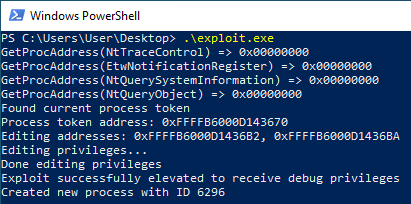
\includegraphics[scale=1]{exploit}
        \caption{Успешный запуск нового процесса}
    \end{figure}
    
\end{frame}

\begin{frame}{Запуск эксплойта}
    
    \begin{figure}[h]
        \centering
        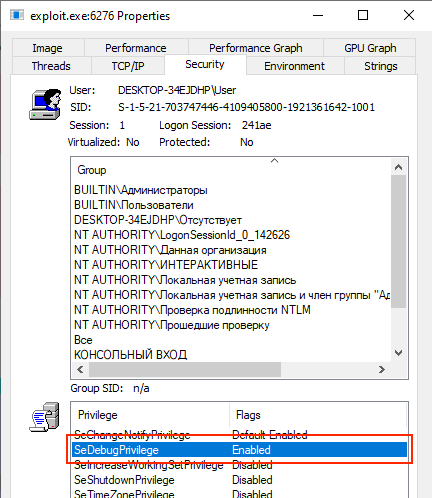
\includegraphics[scale=0.4]{elevated-privileges}
        \caption{Процесс эксплойта имеет привилегию \texttt{SeDebugPrivilege}}
    \end{figure}
    
\end{frame}

\begin{frame}{Новый процесс}
    
    \begin{figure}[h]
        \centering
        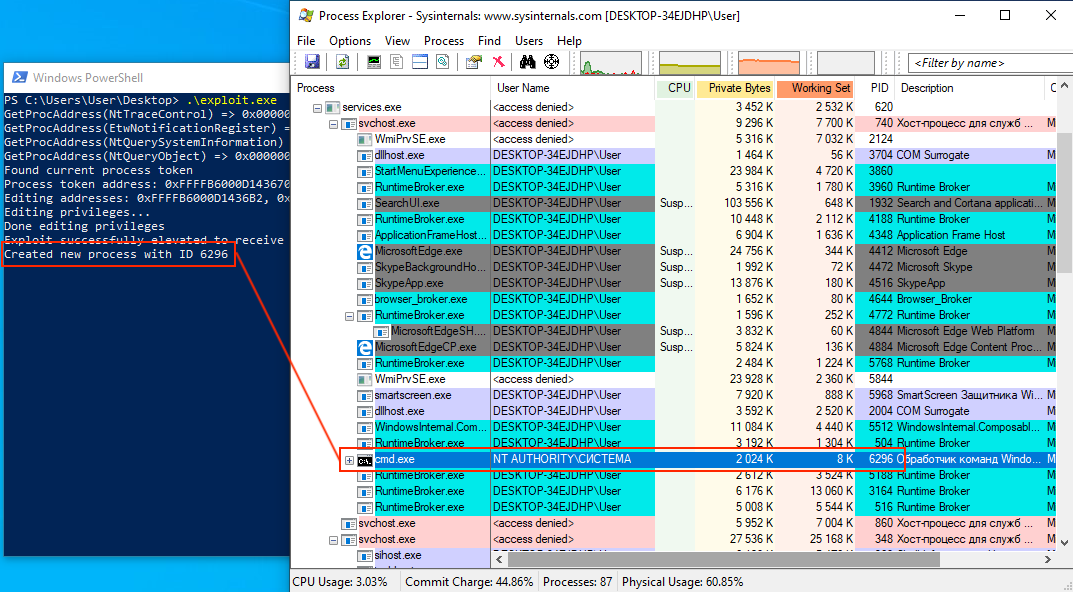
\includegraphics[scale=0.35]{working}
        \caption{Созданный процесс запущен от имени системы}
    \end{figure}
    
\end{frame}


\section{Уязвимые версии системы и меры защиты}

\begin{frame}{Уязвимые версии системы и меры защиты}
    
    \begin{alertblock}{Уязвимые версии Windows}
        Все версии Windows 10 и Windows Server 2019, все сборки до 1909 включительно, а также некоторые 2004.
    \end{alertblock}
    
    \begin{alertblock}{Меры защиты}
        \begin{itemize}
            \item Установить обновление KB4571756 от 8 сентября 2020.
        \end{itemize}    
    \end{alertblock}

\end{frame}


\section{Список использованной литературы}

\begin{frame}{Список использованной литературы}
    
    \begin{enumerate}
        \item Windows Kernel Elevation of Privilege Vulnerability [Электронный ресурс] : 2020. -- Режим доступа: https://msrc.microsoft.com/update-guide/vulnerability/CVE-2020-1034. Дата обращения: 21.03.2022.
        \item Руссинович М., Соломон Д., Ионеску А., Йосифович П. Внутреннее устройство Windows. 7-е изд. -- СПб.: Питер, 2018. -- 944 с.: ил. -- (Серия "Классика computer science").
    \end{enumerate}
    
\end{frame}

\end{document}
